%
	\section{Oxygen Plasma Chemistry}\label{sec:negionphysics}
%
		In comparison to most inert working gases in ccrf discharges, oxygen has an overwhelming number of reaction sets for collisions of elastic, inelastic and reactive character. Additionally, the negative ion species has to be taken into account when discussing collisional processes. For example, an in-depth benchmarking of both simulated and experimentally measured cross section data is given by Gudmundsson et al.\@ in~\cite{Gudmundsson13}. There, 33 collisions and reactions have been revisited, already reducing the investigation to the most important processes in ccrf plasma. In this thesis the selection of possible reactions will be based on~\cite{Bronold07b} and slightly modified. The final collection of cross sections can be found in~\autoref{tab:cross_sections} and observed in~\autoref{fig:cross_sections_mine}. Those data are semi-empirical, meaning part of them are based on measurements in finite energy ranges and low-/high-energy asymptotic models. Cross sections for very high energies are not important, as the collision probability usually decays very fast here.\\
		As already seen in~\autoref{sec:heating}, collisions strongly influence the particle distribution functions and density profiles. Furthermore, a good understanding of the plasma chemistry is key to, e.g.\@ applications in surface physics supported by gas discharges. Of high importance for plasma-assisted material processes is the generation of negative ions. Hence the ratio $\alpha=n\ix{i,-}/n\ix{e}$ is important to characterize the electronegative plasma, like a ccrf oxygen discharge by $\alpha>1$.\\
		I will highlight the most important collisions and reactions in the following section. 
%
		\begin{longtable}{lll}
			\toprule%
				\bfseries Nr. & \bfseries Reaction & \bfseries Type \\%
			\toprule\midrule\endhead%
						& \bfseries Elastic scattering 							& \bfseries Energy loss 	\\% 
						$(1)$  & $e^{-}+O\ix{2}			 	\rightarrow	O\ix{2}+e^{-}$ &						\\%
						$(2)$  & $O^{-}+O\ix{2}			 	\rightarrow	O\ix{2}+O^{-}$ & 						\\%
						$(3)$  & $O\ix{2}^{-}+O\ix{2} \rightarrow	O\ix{2}+O\ix{2}^{-}$ & 			\\ \midrule%
						& \bfseries Electron energy loss scattering & \bfseries Energy loss 	\\%
						$(4)$  & $e^{-}+O\ix{2}			 	\rightarrow	O\ix{2}^{\nu}+e^{-}$ & %
										Vibrational excitation	($\nu=1,\dots,4$)											\\%
						$(5)$  & $e^{-}+O\ix{2}			 	\rightarrow	O\ix{2}(Ryd)+e^{-}$ & %
										Rydberg excitation																						\\%
						$(6)$  & $e^{-}+O\ix{2}			 	\rightarrow	O(1D)+O(3P)+e^{-}$ & %
										Dissociative excitation at $\unit[8,6]{eV}$										\\%
						$(7)$  & $e^{-}+O\ix{2}		 	 	\rightarrow	O\ix{2}%
																					 (a^{1}\Delta\ix{g},b^{1}\Sigma\ix{g})$ & %
										Meta-stable excitaion																					\\ \midrule%
						& \bfseries Electron and ion reactions & \bfseries Creation and loss 	\\%
						$(8)$  & $e^{-}+O\ix{2}^{+}	 	\rightarrow	2\,O$ & %
										Dissociative recombination 																		\\%
						$(9)$  & $O^{-}+O\ix{2}^{+}	 	\rightarrow	O\ix{2}+O$ & %
										Neutralization						 																		\\%
						$(10)$ & $e^{-}+O\ix{2}	 		 	\rightarrow	O+O^{-}$ & %
										Dissociative attachment		 																		\\%
						$(11)$ & $O^{-}+O\ix{2}			 	\rightarrow	O+O\ix{2}+e$ & %
										Direct detachment 																						\\%
						$(12)$ & $e^{-}+O\ix{2}		 		\rightarrow	2e^{-}+O\ix{2}^{+}$ & %
										Impact ionization 																						\\%
						$(13)$ & $e^{-}+O^{-}			 		\rightarrow	O+2e^{-}$ & %
										Impact detachment																							\\%
			\midrule\bottomrule%
			\caption{%
				Most important colilision and reactions in ccrf plasma with the largest cross sections. %
				Empirical and simulated data, which have been included in this simulation are shown in~\autoref{fig:cross_sections}.}\label{tab:cross_sections}	
		\end{longtable}	
%		
		\subsection{Collisions and Reactions}\label{sec:negiondynamics}
%	
			The elastic collisions of $(1)$--$(3)$ conserve the particle numbers. Those are inter-species scattering processes, which will be assumed to have an isotropic inincident angle dependency~\cite{Bronold07b}. Intra-species elastic collisions were not very important at the selected parameter regions, though ion-ion scattering can strongly incluence the IEDF structure of the concerned densities are very high. However, for the electron species a binary \emph{coulomb scattering} process was used: the scattering angle $\chi$ is given by~\autoref{equ:coulomb_scatter} with $v\ix{rel}$ the relative velocity, $\ln\Gamma$ the Coulomb logarithm (see~\autoref{tabe:physicalquantities}) and $\tau\ix{c}$ the collision time.
%
			\begin{align}
				\langle\tan^{2}\frac{\chi}{2}\rangle=\frac{e^{4}n\ix{e}\ln\Gamma}%
					{8\pi\varepsilon\ix{0}m\ix{e}^{2}v\ix{rel}^{3}}\tau\ix{c}%
				\label{equ:coulomb_scatter}	
			\end{align}	
%
			The~\autoref{fig:cross_sections} shows the corresponding cross sections. In fact, only two are elastic processes, where as the collision of $O\ix{2}^{+}$ and the neutral molecule is a charge exchange reaction with momentum transfer. This kind of process:
%
			\begin{align}
				A^{-/+}+B\rightarrow A+B^{+/-}%
				\label{equ:charge_exchange}
			\end{align}
%
			is important for the consideration of surface effects. An ion with greater than thermal velocity coming from the wall will be cooled down by charge exchange collisions, which will transfer heat into the neutral reservior.\\
			Electron energy loss occurs due to inelastic collisions $(4)$--$(7)$, where an oxygen molecule is excited or dissociated into fragments. Here, the spatio-temporal evolution of the molecule or the fragments are of no interest for this thesis. Hence they are treated as `test collisions', in which only the electrons lose momentum and change direction. Again, the neutral particle reservior is considered to equilibrate at a sufficiently short time scale $<\unit[\tenpo{-15}]{s}\,$. The isotropic post-collision relative velocity change in the center-of-mass system gives
%
			\begin{align}
				\widetilde{v}\ix{rel}=\sqrt{v\ix{rel}^{2}-\frac{2\Delta E}{\mu\ix{i,j}}}\,.%
				\label{equ:electron_energyloss}
			\end{align}
%
			The most important electron energy loss scattering is the vibrational and electronic excitation, as well as the dissociation iof the oxygen molecule.\\
			The last class of collisions concerned here are the electron and ion production processes. Collisions $(8)$ and $(9)$ are the annihilation of the two oppositely charge particles. Those are namely recombination processes. The ion-ion neutralization is constructed by a \emph{Landau-Zener} model, where the adiabatic energy of the ($O^{-}$,$O\ix{2}^{+}$) configuration decreases when the particles approach each other. At the critical distance $R\ix{c}$ this energy drops bellow the one of the ($O$,$O\ix{2}$) configuration, yielding the probability to change states $\sigma\ix{r}(E)$ 
%
			\begin{align}
				\sigma\ix{r}(E)=4\pi R\ix{c}^{2}\left(1+\frac{1}{R\ix{c}E}\right)\,.%
				\label{equ:neutralization}
			\end{align}
%			
			The dissociative attachment $(10)$ and direct detachment $(11)$ are treated as binary collisions, like the elastic electron scatter process. In the experiment there is a second stage for the direct detachment process: through associative detachment, oxygen atom, electron and molecule form an ozone $O\ix{3}$ particle. This most likely due to the presence of meta-stable $O\ix{2}(a^{1}\Delta\ix{g})$. After the necessary threshold energy of $\unit[1,3]{eV}$ has been supplied to directly detach $O^{-}$ on an oxygen molecule, the afore-mentioned detachment takes no energy whatsoever, making it a potentially important loss channel for cold $O^{-}$ ions.\\
			For impact ionization $(12)$ and detachment $(13)$ the following is assumed: first, an inelastic binary collision takes place, in which the electron loses the necessary reaction energy. The post-collision oxygen particle is afterwards split into an additional $e^{-}$ and atom/ion ($O^{-}$/$O$), which proceed to perform an elastic binary collision. During this process, energy and momentum conservation is satisfied, ensuring numerical stability.\\

%			
			\begin{figure}[!b]
				\centering
				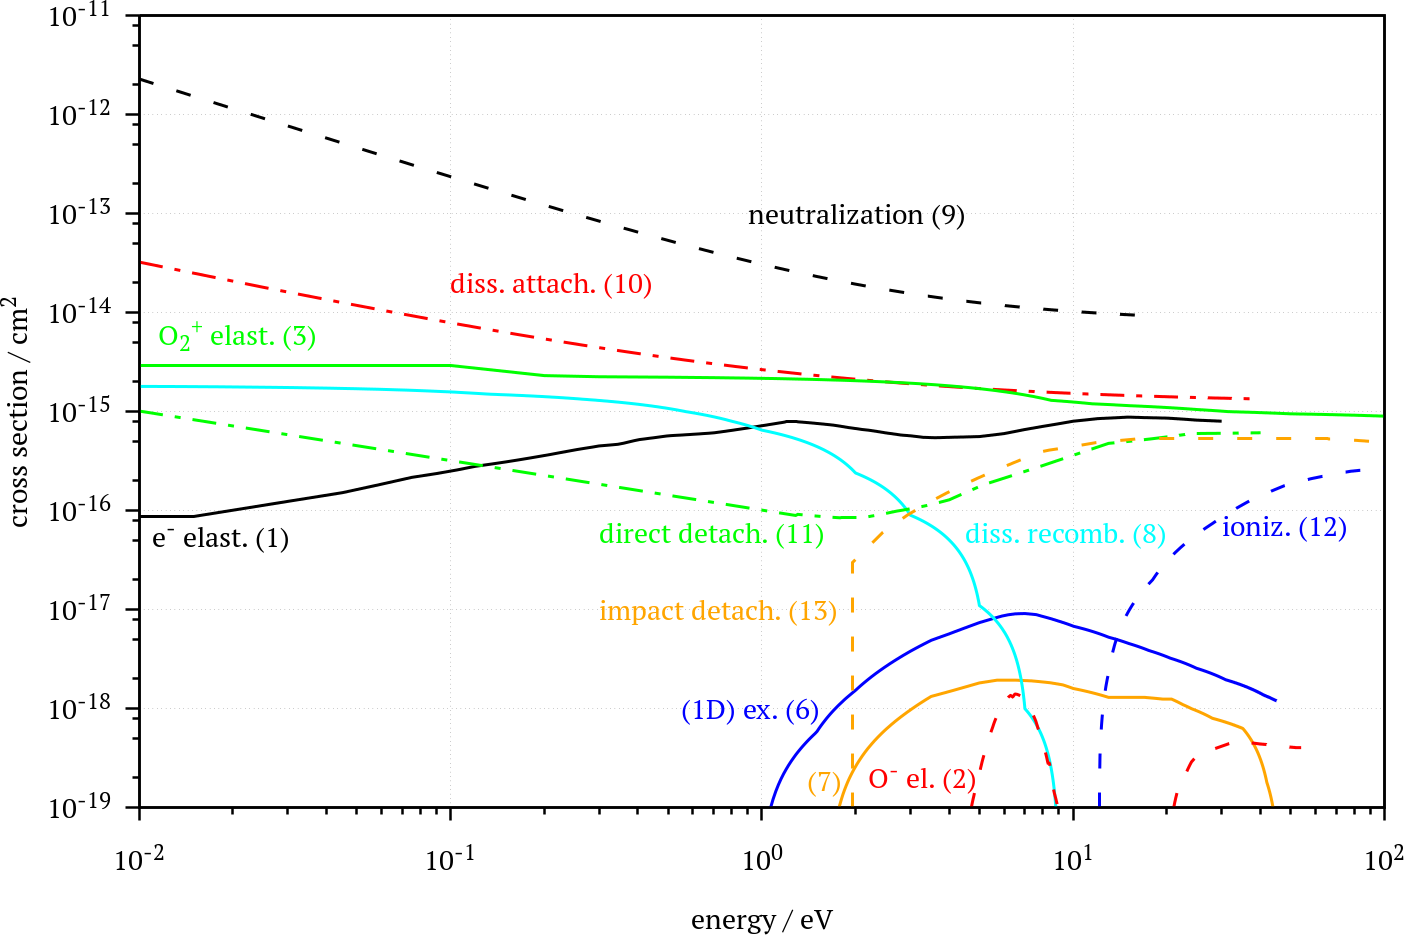
\includegraphics[width=1.0\textwidth]{figures/xsections.png}
				\caption{%
					Test.}%
				\label{fig:cross_sections}	
			\end{figure}	
%			
		\subsection{Anion Species}\label{sec:anionproduction}
%
			The main production channel of negative oxygen ions in ccrf disharges at low pressures and temperatures is the dissociative attachment reaction $(10)$. Here, an electron becomes attached to a molecule. The successive electronic excitation is of short duration and does not change the intra-molecular distance. Afterwards, theres a significant chance of transition to a dissociative state exists, which has a lower equilibrium energy at greater intra-nuclear distances. Hence, the dissociation of this molecule is rather likely.
%
			\begin{align}
				e^{-}+AB\rightarrow A+B^{-}%
				\label{equ:dissociative_attach}
			\end{align}
%
			Another possible creation channel is a three-body collision of non-dissociative character, whose cross sections are magnitudes smaller than those of \autoref{equ:dissociative_attach}. Hence I will only consider dissociative attachment reactions $(10)$ for the anion production.\\
			Negative ion loss can happen through reactions $(11)$, $(13)$ and $(9)$. The latter is the only collision which has a cross section larger than the creation via dissociative attachment (see~\autoref{fig:cross_sections}). For all relative energies, the neutralization has a probability about one magnitude larger. Cross sections of direct $(11)$ and impact $(13)$ detachment are, depending on the energy, about one to two orders of scale smaller.\\
			In general, produced negative ions are cold. It is found that the anion distribution reaches until the boundaries of the bulk, where processes with large cross sections at low energies become important~\cite{Bronold07b}. Those would be ion-ion neutralization and associative detachment. Direct detachment, though being still present around $E<\unit[1]{eV}$, has an energy threshold and is not significant for this region. Furthermore, the probability of neutralization $(9)$ is proportional to the $O\ix{2}^{+}$-density. Bronold et al.\@ proposes, that the production and loss of $O^{-}$ is rather insensitive to voltage changes up to $\unit[300]{V}$. Furthermore, the most important range for incident energies will be $4$--$\unit[15]{eV}$, while the EEDF is rather voltage-independent.
			Considering the physics of a negative ion --- $O^{-}$ follows the same dynamic and kinetic behaviour as the electrons, but is easily confined by the plasma potential due to their much greater mass and, hence $\omega\ix{p,i-}<<\omega\ix{p,e}$ --- the main loss and production channels are most prominent in the bulk. Therefore, a low-pressure, low-temperature ccrf discharge has an electronegative core, in which the cold anions are, and areas where they are excluded. The presence of negative ions also has a great impact on the distribution functions of other plasma species. It is possible to form a quasi-neutral volume core, consisting only of ion species, and a peripheral electron-ion plasma in the discharges sheaths. At pressures $>\unit[30]{Pa}$ and large input powers, the value of electronegativity $\alpha$ leads to instabilities between ionization and electron attachment reactions. The electron density peaks, where as the corresponding temperatures drops. Because of the strong negative ion coupling, the $O^{-}$ density fluctuates as well.
